%
% fvm.tex
%
% (c) 2020 Prof Dr Andreas Müller, Hochschule Rapperswil
%
\begin{frame}[fragile]
\frametitle{Finite Volumina}
\begin{block}{Idee}
Funktionswerte durch Integrale/Mittelwerte ersetzen
\end{block}
\vspace{-15pt}
\begin{columns}[t]
\begin{column}{0.56\hsize}
\uncover<2->{%
\begin{block}{1-dim Strömungsproblem}
$\varrho=\mathstrut$ Dichte,
$f=\mathstrut$ Stromdichte
\[
\frac{\partial\varrho}{\partial t} + \frac{\partial f}{\partial x} = 0
\]
(Kontinuitätsgleichung)
\end{block}}
\uncover<3->{%
\begin{block}{Mittelwerte über Intervalle}
\vspace{-15pt}
\begin{align*}
{\color{blue}
\bar{\varrho}_i(t)} &= \int_{i}^{i+1} \varrho(t,x)\,dx
&&\text{Masse im Interval}
\\
\uncover<4->{%
{\color{red}
\bar{f}_j(x)}}&\uncover<4->{= \int_{j}^{j+1} f(t,x) \,dt
&&\text{Verlust durch $x$}}
\end{align*}
\end{block}}
\end{column}
\begin{column}{0.40\hsize}
\begin{center}
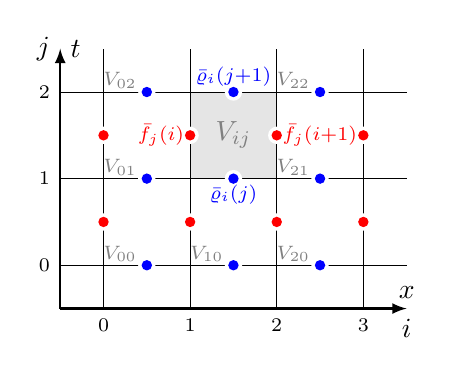
\begin{tikzpicture}[>=latex,thick,scale=1.1]

\fill[color=gray!20] (1,1) rectangle (2,2);

\def\volumen#1#2{
	\node[color=gray] at ({#1-0.12},{#2-0.08}) [above right] {$\scriptstyle V_{#1#2}$};
}

\volumen{0}{0}
\volumen{1}{0}
\volumen{2}{0}

\volumen{0}{1}
\volumen{2}{1}

\volumen{0}{2}
\volumen{2}{2}

\node[color=gray] at (1.5,1.5) {$V_{ij}$};

\foreach \x in {0,...,3}{
	\draw[line width=0.2pt] (\x,-0.5)--(\x,2.5);
	\node at (\x,-0.5) [below] {$\scriptstyle \x$};
}
\foreach \y in {0,...,2}{
	\draw[line width=0.2pt] (-0.5,\y)--(3.5,\y);
	\node at (-0.5,\y) [left] {$\scriptstyle \y$};
}
\uncover<4->{
	\foreach \x in {0,...,3}{
		\foreach \y in {0,...,1}{
			\fill[color=white] (\x,{\y+0.5}) circle[radius=0.10];
			\fill[color=red] (\x,{\y+0.5}) circle[radius=0.06];
		}
	}
	\node[color=red] at ({1+0.05},1.5)
		[left] {$\scriptstyle \bar{f}_j(i)$};
	\node[color=red] at ({2-0.05},1.5)
		[right] {$\scriptstyle \bar{f}_j(i+1)$};
}
\uncover<3->{
	\foreach \x in {0,...,2}{
		\foreach \y in {0,...,2}{
			\fill[color=white] ({\x+0.5},\y) circle[radius=0.10];
			\fill[color=blue] ({\x+0.5},\y) circle[radius=0.06];
		}
	}
	\node[color=blue] at (1.5,{2-0.05})
		[above] {$\scriptstyle \bar{\varrho}_i(j+1)$};
	\node[color=blue] at (1.5,{1+0.05})
		[below] {$\scriptstyle \bar{\varrho}_i(j)$};
}
\draw[->] (-0.5,-0.5)--(3.5,-0.5) coordinate[label={$x$}];
\node at (3.5,-0.5) [below] {$i$};
\draw[->] (-0.5,-0.5)--(-0.5,2.5) coordinate[label={right:$t$}];
\node at (-0.5,2.5) [left] {$j$};

\end{tikzpicture}
\end{center}
\vspace{-10pt}
\uncover<5->{%
\begin{block}{Differenzengleichung für $V_{ij}$}
\vspace{-15pt}
\[
\bar{\varrho}_i(j+1) - \bar{\varrho}_i(j)
=
\bar{f}_j(i+1)-\bar{f}_j(i)
\]
\end{block}}
\end{column}
\end{columns}
\end{frame}
